\documentclass[FM,RP]{tulthesis}
% tento dokument používá balíky specifické pro XeLaTeX a lze jej přeložit
% jen XeLaTeXem, nemáte-li instalována použitá (komerční) písma, změňte
% nebo vymažte příkazy \set...font na následujících řádcích

\newcommand{\verze}{1.7}

\usepackage{polyglossia}
\setdefaultlanguage{czech}
\usepackage{xevlna}

\usepackage{makeidx}
\makeindex

% fonty
\usepackage{fontspec}
\usepackage{xunicode}
\usepackage{xltxtra}
\usepackage{graphicx}
\usepackage{pdfpages} 


% příkazy specifické pro tento dokument
\newcommand{\argument}[1]{{\ttfamily\color{\tulcolor}#1}}
\newcommand{\argumentindex}[1]{\argument{#1}\index{#1}}
\newcommand{\prostredi}[1]{\argumentindex{#1}}
\newcommand{\prikazneindex}[1]{\argument{\textbackslash #1}}
\newcommand{\prikaz}[1]{\prikazneindex{#1}\index{#1@\textbackslash #1}}
\newenvironment{myquote}{\begin{list}{}{\setlength\leftmargin\parindent}\item[]}{\end{list}}
\newenvironment{listing}{\begin{myquote}\color{\tulcolor}}{\end{myquote}}
\sloppy

% deklarace pro titulní stránku

\TULtitle{Vytvoření výukové aplikace řešící blokové diagramy bezporuchovosti (RBD)}{}
\TULprogramme{B2646}{Informační technologie}{}
\TULbranch{1802R007}{Informační technologie}{}
\TULauthor{Jan Špecián}
\TULsupervisor{Ing. Josef Chudoba, Ph.D.}
\TULyear{2019}

\begin{document}
%\ThesisStart{pic/zadaniBPScan.pdf}
\ThesisStart{male}
%\includepdf[scale=1,angle=0,pages=-]{pic/prohlaseni.pdf} 

\begin{abstractCZ}
    Práce je zaměřena na tvorbu desktopové aplikace pro tvorbu RBD diagramů a spojených výpočtů a vyzualizací.
\end{abstractCZ}

\begin{keywordsCZ}
    RBD
\end{keywordsCZ}

\vspace{2cm}



\clearpage

\begin{acknowledgement}
    Tímto bych rád poděkoval Ing. Josef Chudobovi, Ph.D. za věnovaný čas v konzultacích a odborné vedení plné trpělivosti a s tím spojené nabyté zkušenosti.
\end{acknowledgement}

\tableofcontents
\listoffigures

\clearpage

\begin{abbrList}
    \textbf{JSON} & JavaScript Object Notation \\
    \textbf{LINQ} & Language Integrated Query \\
    %\textbf{PDF} & Portable Document Format \\
   
\end{abbrList}

\chapter*{Úvod}
    U každého systému je velmi důležitá jeho funkční spolehlivost během doby jeho životnosti. Každý systém, pokud má existovat a fungovat co nejdéle a přitom bez závad,
    nebo alespoň s jejich co nejmenším počtem, musí splňovat jednu zásadní vlastnost, a tou je spolehlivost. 
    Požadavek na dostatečně velkou a často až maximální spolehlivost námi užívaných systémů má tudíž zcela zásadní význam z hlediska bezpečnostního, ekonomického i
    ekologického. 

    Cílem ročníkového projektu je navrhnout a implementovat desktopovou aplikaci pro tvorbu a jednoduchou vizualizaci RBD diagramů a výpočet parametrů spolehlivosti.
    Zobrazit střední dobu do poruchy pro každý blok a poskytnout možnost vizualizace distribuční funkce pro každý blok v kombinace sérriového a paralelního zapojení bloků.

\chapter{Přehled existujících softwarových nástrojů}

\chapter{Teoretický úvod}
        
    \section{Distribuční funkce}

    \section{Exponenciální rozdělění}

    \section{Spolehlivost a střední doba mezi poruchami}
        \subsubsection{Střední doba mezi poruchami}
            Základní veličinou pro měření spolehlivosti systému je střední doba mezi poruchami (MTBF, Mean Time
            Between Failure). Obvykle je udávána v hodinách. Čím vyšší je hodnota MTBF, tím vyšší je spolehlivost
            produktu.\cite{3}
            Je statistická veličina používaná ke kvantifikaci spolehlivosti součásti, či celého výrobku.
            Určuje se pro výrobek nebo zařízení, které se opravuje. \cite{3}
        \subsubsection{Spolehlivost}
            Spolehlivost je schopnost systému nebo součásti vykonávat požadované funkce za daných
            podmínek po určené časové období \cite{4} 

            $$ Spolehlivost = e^{-(\frac{Time}{MTBF})}$$
    
    \section{Analýza blokového diagramu bezporuchovosti (RBD)}

        Analýza blokového diagramu bezporuchovosti (RBD - Reliability Block Diagram) je metoda analýzy systému. 
        Diagram RBD je grafická reprezentace logické struktury systému v podobě podsystémů a/nebo součástí. 
        To umožňuje, aby byly cesty úspěchu (funkceschopného stavu) reprezentovány tak, jak jsou bloky (podsystémy/součásti) logicky propojeny.\cite{1}

        Blokové diagramy jsou mezi prvními úkoly dokončenými během etapy vymezení produktu. 
        Mají být vypracovány jako součást vývoje počáteční koncepce. 
        Práce na nich mají být zahájeny, jakmile existuje vymezení programu, a mají být dokončeny jako součást analýzy požadavků a 
        mají se neustále rozšiřovat do větších úrovní podrobnosti, 
        jakmile budou k dispozici data, aby bylo možné činit rozhodnutí a provádět optimalizace nákladů a přínosů.\cite{2}

    \section{Základní zapojení bloků}
        \subsubsection*{Sériové zapojení}
            Při poruše jedné komponenty dojde k poruše celého systému. 
            Systém je v bezporuchovém stavu, pokud všechny jeho komponenty nemají poruchu.\cite{5}
            \begin{figure}[h]
                \centering
                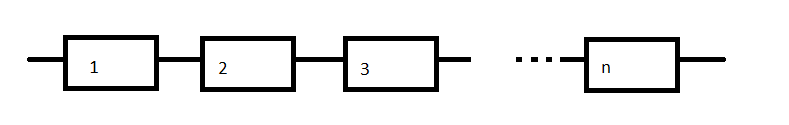
\includegraphics[scale=0.75]{pic/seriove.png}
                \caption{Příklad sériového zapojení komponent} \label{Obrázek č. 2.1}
            \end{figure}

        \subsubsection*{Paralelní zapojení}
            K poruše celého systemu dochází pokud jsou v poruše všechny jeho komponenty. Bezporuchový stav trvá, dokud je alespoň jedna komponenta v bezporuchovém stavu.
            Z hlediska odhadu pravděpodobnosti představuje paralelní systém nejlepší variantu pro odhad pravděpodobnosti bezporuchového stavu.\cite{5}
            \begin{figure}[h]
                \centering
                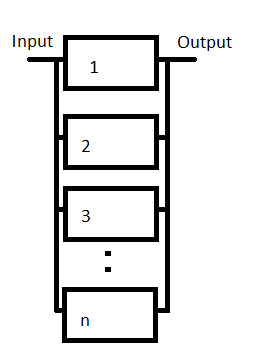
\includegraphics[scale=0.75]{pic/paralelni.png}
                \caption{Příklad paralelního zapojení kopmonent} \label{Obrázek č. 2.1}
            \end{figure}

\chapter{Návrh desktopové aplikce .NET}
    \section{Objektová struktura}

    \section{Pomocné třídy}

\chapter{Průběh vývoje}
    \section{Rozdělení projektu na subprojekty}
    \section{}
\chapter{Testování}

    Pro testování funkčních bloků byla použita výchozí knihovna pro Unit testování v prostředí .NET pro desktopové aplikace MSTest.
    Za pomoci testování jsem došel ke správným výsledkům za pomoci připravené konfigurace a tím jsem ušetřil práci manuálním testováním.
    Další nespornou výhodou testování je odhalení chyb při změně tím,  že testovací metody odhalí neočekávané výledky.

    Testované byly třídy pro výpočet distribuční funkce.

\chapter{Návod k použití}

    Pro spuštění aplikace pro vývoj je potřeba mít nainstalované Visual Studio 2017 a novější. V přiloženém CD ve složce SpecianPRJ spusťte soubor SpecianPRJ.sln. 
    Pro standartní spuštění aplikace stačí otevřít soubor s příponou .exe.

    Pro obě varianty spuštní je nutným předpokladem nainstalovaný plný .NET Framework 4.6.1 a novější. 

    \section*{Založení nového diagramu}
    \section*{Uložení a otevření nového diagramu}
    \section*{Přidání prvku}
    \section*{Výpočty}

\chapter{Závěr}



\begin{thebibliography}{Mm99}
    \bibitem{1}
        28.6.2007, Prof. Ing. Václav Legát, DrSc., Zdroj: Verlag Dashöfer
    \bibitem{2}
        %https://theses.cz/id/dnvmwp/downloadPraceContent_adipIdno_11870
    \bibitem{3}
        http://gabben.wbs.cz/mtbf1.pdf
    \bibitem{4}
        IEEE 90
    \bibitem{5}
        %file:///C:/Users/King/Documents/PRJ/skripta/Plzen_06_10_2005.pdf
\end{thebibliography}

\end{document}
